\documentclass{article}
\usepackage{amsmath}
\usepackage{amssymb}
\usepackage{graphicx}
\usepackage{hyperref}
\usepackage[version=4]{mhchem}

\title{Example 1}
\date{}

\begin{document}
\maketitle

Circle \(O\) is inscribed in equilateral triangle \(A B C\). Circle \(P\) of radius 1 is tangent to circle \(O\) and segments \(A B\) and \(B C\). Find the area of triangle \(A B C\).\\
(A) 27\\
(B) \(9 \sqrt{3}\)\\
(C) \(36 \sqrt{3}\)\\
(D) \(27 \sqrt{3}\)\\
(E) 47

Solution: (D).\\
Draw \(P F \perp A B\) and \(O E \perp A B\).\\
\centering
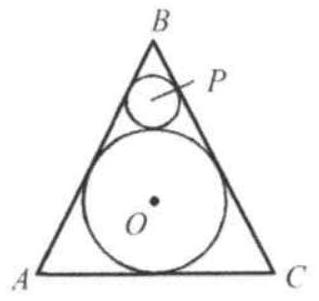
\includegraphics[width=\textwidth]{images/problem_image_1.jpg}

Connect \(B D\).\\
Triangle \(B E O\) is a \(30^{\circ}-60^{\circ}-90^{\circ}\) triangle and \(B P=2 P F=2\).\\
Let \(O E=r\).\\
We know that \(B O=2 O E \quad \Rightarrow \quad 2 r=r+3 \quad \Rightarrow r=3\)\\
We know that \(r=\frac{1}{6} a \sqrt{3}\), where \(a\) is the length of the side of triangle \(A B C\). So \(3=\frac{1}{6} a \sqrt{3} \quad \Rightarrow \quad a=6 \sqrt{3}\)\\
We know that \(S_{\triangle A B C}=\frac{1}{4} a^{2} \sqrt{3}\). So\\
\centering
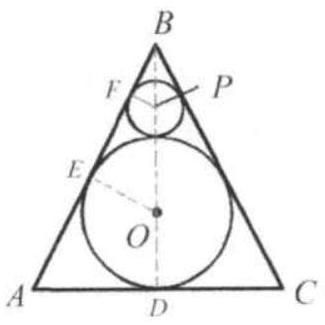
\includegraphics[width=\textwidth]{images/reasoning_image_1.jpg}\\
\(S_{\triangle A B C}=\frac{1}{4} \times(6 \sqrt{3})^{2} \sqrt{3}=27 \sqrt{3}\)\\

\end{document}
